\section{Part B}
%=========================Intro====================================%
So far the characterization of the graphics card performance was in terms of the speed of operations. Now we turn to characterize the quality, specifically the precision of the native arithmetic operations. Precision is crucial because the speed render irrelevant if the results are not accurate. Even under the IEEE-754 Standards, identical operations could produce different results when executed on two different machines because of different hardware implementation and the peculiar nature of floating points operations (e.g. floating point addition is not associative). 

In this section, we start by quantifying the error of the native arithmetic operations. We compare GPU's results with the CPU to measure the error. We also try to discover a precision-related undocumented features; how rounding is implemented in our graphic card. 

%=========================Arithmetic Opt====================================%
\subsection{Arithmetic Operations Accuracy:}
Here we test a range of basic float point arithmetic operation offered by the GPU. Taking the CPU results as our datum, the absolute relative error between the GPU's results and CPU's results represents the GPU errors. The rationale behind this method is that both CPU and GPU are compliant with IEEE-754 Standard. %We will revisit this idea in Section \ref{sec:dot}, where we see careful implementation could make the graphic card more accurate. 
Our approach was to write an OpenGl code that utilizes fragment shaders to perform the arithmetic operations. Basically, we send floating point value to the GPU as a color component of pixels, then perform a basic operation on it, and finally we can read the pixel's final color component that we applied the shader to. Initially we wanted to use GLSL to write our fragment shader; however, we wanted to directly access the GPU hardware to eliminate any source of error that may stems from different software configurations or optimization. That's why we decided to use Shader Assembly Language ARB to impelment our fragment shader. That way we can guarantee that the GPU is only doing precisely what we ask it to do (eg: calculating the Sin of a number). Using ARB instructions, we were able to quantify the error in Sin, Cos, Power, Log, and Square root functions. 


\begin{figure}[!tbh]
 \centering  
    {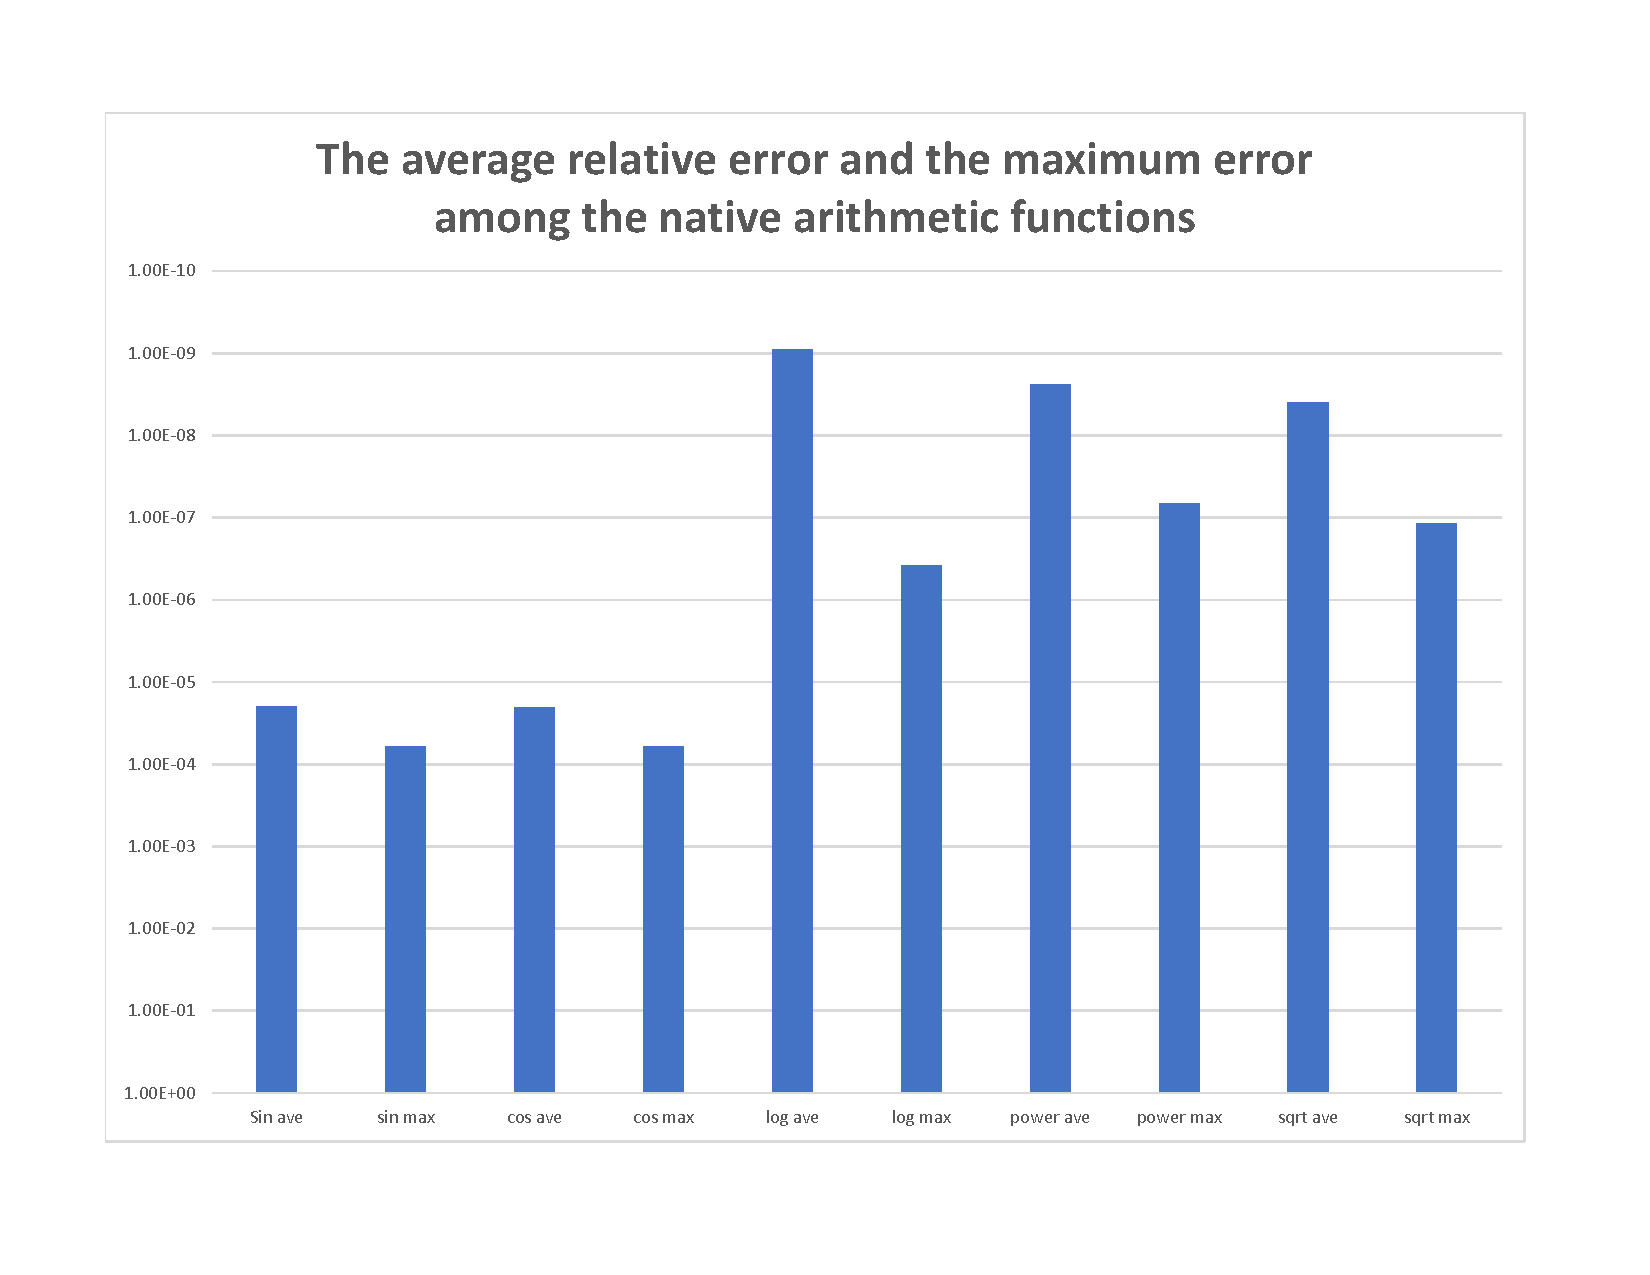
\includegraphics[width=1.0\linewidth]{fig/histogram_comparison.pdf}}    
  \caption{The average of the realative error and the maximum error between the native arithmetic function that we tested }
   \label{fig:histogram_comparison}
\end{figure} 

We conduct the test for each of our functions by giving it a series of inputs starting from 0.1 and ending at 100 with an increment of 0.01 between each input values. Then we calculate how much the GPU results deviate form the CPU results and average that thoughout our iterations. Also we keep track of the maximum instance of error to give us an idea of how bad the worest case scenario can be. From figure 5 we can conclude that the sinusoidal fuction usually have higher error on our GPU. The average relative error for Sin was the highest among all fuctions also it had the worest case scenario ever. On the other hand the logarithmic function had the least error among all functions. However, the maximum value of the error of the log function was almost 1000 times as much as the average case. We can infer that the GPU implementation of the log is not as reliable as the other fuctions since some time its precision can vary dramatically.

\begin{figure}[!tbh]
 \centering  
 \subfloat[ ]
   {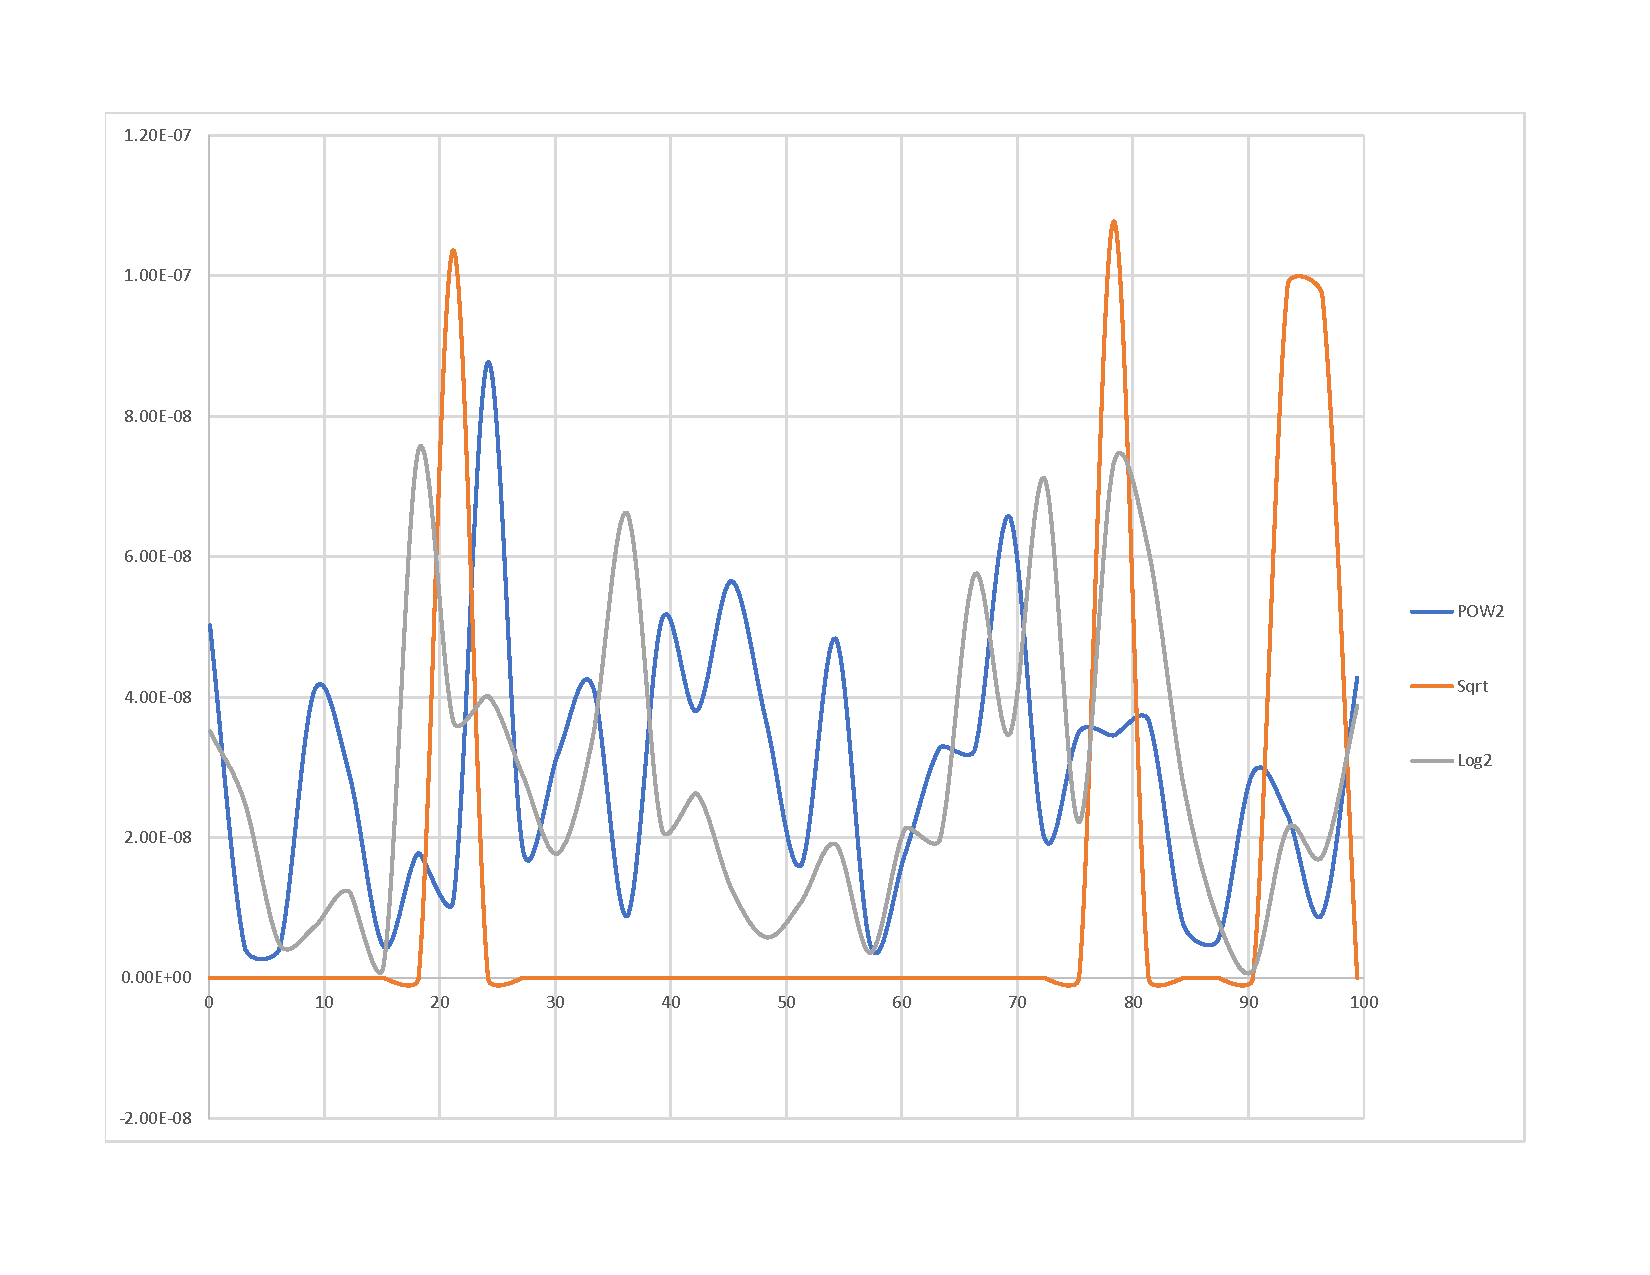
\includegraphics[width=0.49\linewidth]{fig/error_trend1.pdf}}
 \subfloat[ ]
    {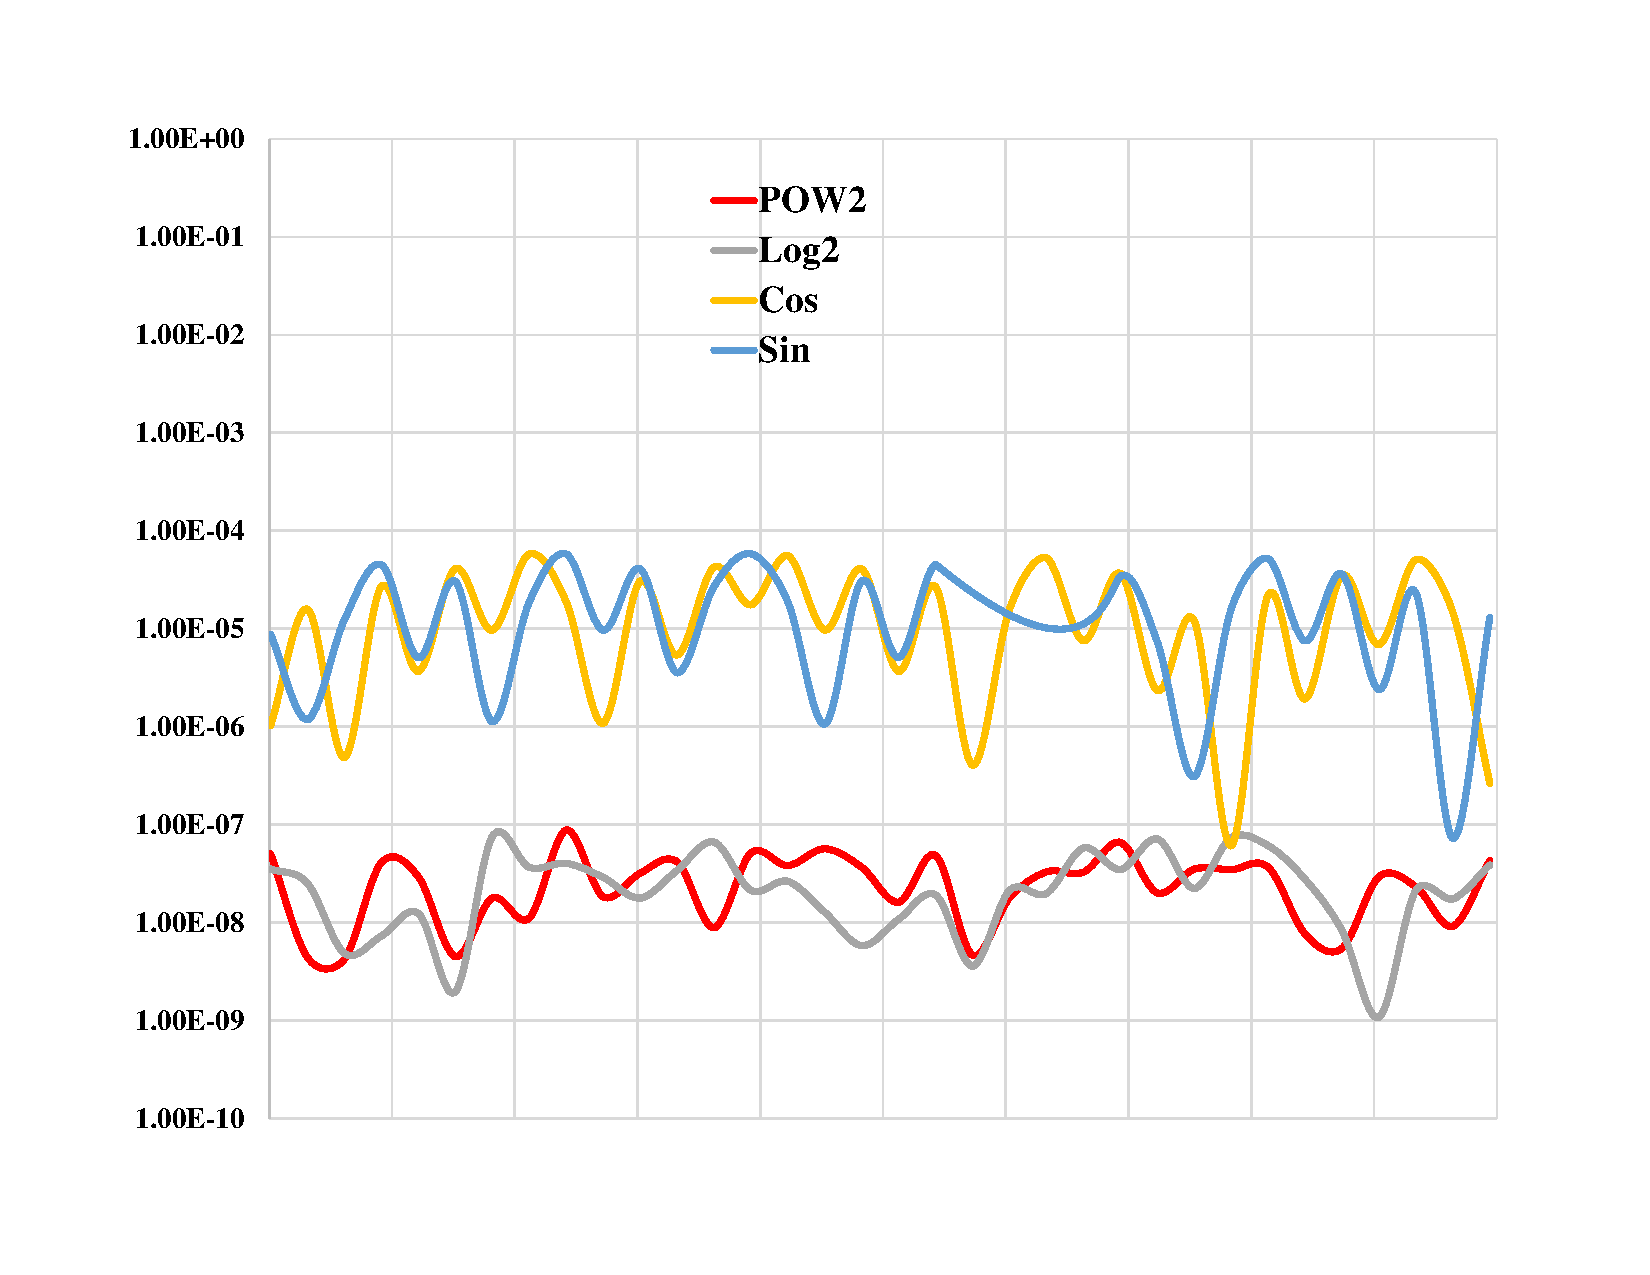
\includegraphics[width=0.49\linewidth]{fig/error_trend2.pdf}}    
  \caption{The error trend accross our testing space }
   \label{fig:fill_geo3}
\end{figure}

Another important metric that we need to examine is how the precision of each of our operations get affected by increasing the value on the input. In other words, we need to figure our if there is a certain trend for the error in each our functions. Figure 6 shows samples of the relative error throughout our testing space. 


%=========================Dot Product====================================%
%\subsection{Dot Product}\label{sec:dot}
%Here we performance dot product between two float vectors and measure the error between the 
%\cite{whitehead2011precision}

%=========================Rounding====================================%
\subsection{Detect Precision via Shader Program}
The purpose of this test is to first verify that our GPU is IEEE-754 compliant and second to identify the rounding algorithm implemented. For this test, we borrowed the fragment shader used in Russell's article \cite{stuart2013mobile} shown in Figure \ref{fig:shader_code}. In Russell's article, the shader was used to benchmark the accuracy of GPU floating point across different mobile GPUs. 

\subsubsection{Compliance with IEEE-754}
The shader simply fills the screen with 26 bars. Given infinite precision, each bar should vary linearly from white (left) to black (right) as a function of $X$ coordinate of the pixel. Note that the implementation calculates $1_X$ so we, instead, can consider $X=0$ is to the left of the screen and $X=1$ is to the right. The shader is written such that with each level/bar, one bit of the fraction (significand) is thrown away. For each level $L$, we add $2^{L}$ to the computed gray value ($X$ coordinate of the pixel) and take the fraction of the result. The added integer ($2^{L}$) does not affect the value of the gray scale, but only its precision. For example, for the first bar, we add  $2^{L}=(1)_{ten}=(1)_{two}$ which is represented by one bit. Thus, when added to $fract(x)$ and taking the $fract()$ of the result, we only loss one bit of the gray scale value's precision. For the next level, we add $2^{L}=(4)_{ten}=(10)_{two}$, which is represented by two bits and thus two bits loss in precision. This goes up till we end up with zero precision in the fraction part and thus the image turns to black. Figure \ref{fig:shader_fig} shows the result of running the shader on our graphic card. We can see that even though we are trying to draw 26 bars, only 23 bars are shown and the rest are black. This verifies that the fraction part (significand) of float point numbers in our graphic card is represented by 23 bits which matches exactly what IEEE-754 requirements. 

\begin{figure}[t!]
\centering
\begin{minipage}[t]{\textwidth}
\centering
\begin{lstlisting}[label=list:ExampleShader,
escapechar=|,
caption={
  Fragment Shader.
}]
void main(void) {
  float y = (gl_FragCoord.y / y_res) * 26.0
  float x = (1.0 -(gl_FragCoord.x / x_res))
  float yp = pow(2.0, floor(y))
  float fade = fract(yp + fract(x))
  if (fract(y) < 0.9)
     gl_FragColor = vec4(vec3(fade), 1.0)
  else
     gl_FragColor = vec4(0.0)
}
|
\end{lstlisting}
\end{minipage}

\caption{The fragment shader implementation for verify the floating-point representation compliance with IEEE-754 standards}
\label{fig:shader_code}
\end{figure}


\begin{figure}[t!]
 \centering   
    {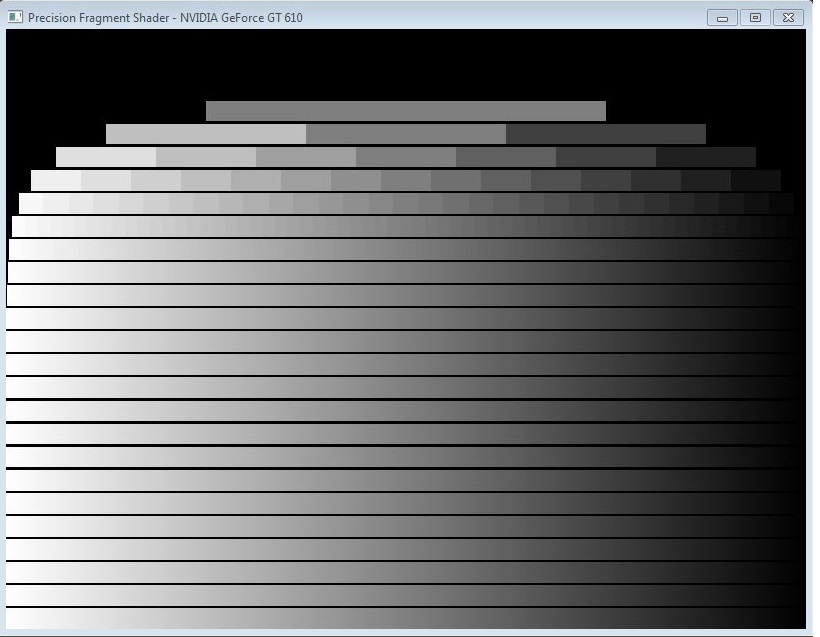
\includegraphics[width=\linewidth]{fig/shader_gt610.JPG}} 
% \subfloat[Precision Shader on Integrated GPU]
%   {\includegraphics[width=0.49\linewidth]{fig/shader_integrated.png}}   
  \caption{Results of applying shader in Figure \ref{fig:shader_code}.}
   \label{fig:shader_fig}
\end{figure} 

\subsubsection{Rounding Algorithm}
We notice on the Figure \ref{fig:shader_fig} that for the last few upper bars that the linearly-varying gray scale is a little edgy. We believe that this is due to rounding. Next we explain why we believe so and we use this to investigate the type of rounding algorithms that is used in our graphic card and compare it with an Intel-integrated graphic card. 

Due to limited finite bits we have to store intermediate values during the calculation in with floating-point numbers, we must do rounding to these values. There are many modes of rounding available; rounding down (truncate), round up, and round to nearest even. Rounding up or down is straightforward and less complicated and thus it is more favorable for embedded system since more emphasis is on the speed than quality.  The IEEE-754 requires the floating-point rounding to be nearest even. This requires storing few (three) extra bits to (guard, round and sticky bit) in order to keep track of the shifted bits \cite{patterson2013computer}. This offers more accurate results such that the guard and round bits will, while shifting, keep track of the two most significant bits to be truncated. Sticky bit can be considered as logic bit that is set to 1 when there is nonzero bits after the round and guard bits. 

Looking again at Figure \ref{fig:shader_fig}, the last visible bar will have only one bit in the significand to represent it. The range of values we need to represent using this value is from 0.000 up 0.9999... in decimals. For the value between $0.00-0.25$, the guard bit is zero. Thus, regardless to the round and sticky bits, the number will be rounded down to 0. This simply means we do nothing or truncate. Since the most significant bit is zero, then we will end up with $0.0$. This explains why the bar at the beginning is black. For values between $0.25-0.5$, the guard bit is now one and the result will depend on the round and sticky bit. Since the stick bit is set, then we will round up (add one to the most significant bit). This gives a value of $(0.5)_{ten}=(0.1)_{two}$ which is gray as the figure shows. Next for value between $0.5-0.75$, the guard bit is now zero again which means we round down (do nothing). Since the most significant bit is one, we will end up with $0.5$. The range between $0.25-0.75$ will result in a most significant bit to be one which gives a gray color. For range between $0.75-0.99$, the guard and stick bit are not set and we will have to round up. Since now the most significant bit is one, adding one to it (rounding up) will result into moving to the next integer and zero in the most significant bit. This explains why the bar turns black at the end. 

 





